%%%%%%%%%%%%%%%%%%%%%%%%%%%%%%%%%%%%%%%%%%%%%%%%%%%%%%%%%%%%%%%%%%%%%%
% Fichero: PrincipalTFG.tex
% Autor: Rubén Márquez Villalta
% Fecha (creación): Febrero 2020 
% Descripción: Documento principal de la memoria del TFG
% Universidad: Escuela Superior de Informática, UCLM(Ciudad Real)
% Titulo: “Global-Manager: Entrenando mediante un Juego Serio a los 
% Jefes de Proyecto en los Desafíos del Desarrollo Global del Software”
%
% ##### Compilación #####
%
% Este documento ha sido desarrollado para compilarse con `pdflatex`,
% `biblatex` (bibliografía con `biber`).
%
% Para su compilación se aconseja utilizar `latexmk` (requiere para su 
% ejecución de un intérprete [`Perl`](http://strawberryperl.com/)):
%
% <\$> latexmk -pdf -silent -synctex=1 --enable-write18 
%
%%%%%%%%%%%%%%%%%%%%%%%%%%%%%%%%%%%%%%%%%%%%%%%%%%%%%%%%%%%%%%%%%%%%%%

% --------------------------------------------------------------------
%
% PREÁMBULO DEL DOCUMENTO TFG
%
% --------------------------------------------------------------------

% ----- Clase del documento (book) -----
\documentclass[
	11pt,			% Tamaño de letra
	a4paper,		% Tamaño de papel
	twoside,		% Impresión a doble cara
	openright,		% Apertura del capítulo a la derecha
	final			% Versión final
]{book}


% ----- Importación de paquetes -----
\usepackage[utf8]{inputenx}			% Codificación de entrada: utf8
\usepackage[english,spanish]{babel}	% Idioma del documento

% ## Geometría de las páginas del documento
\usepackage[		% Márgenes del documento
	top=2.5cm,		% Margen superior
	bottom=2.5cm,	% Margen inferior
	inner=3.5cm,	% Margen al interior
	outer=2cm		% Margen al exterior
]{geometry}

% ## Tipografía
\usepackage[tt=false]{libertine} 	% Libertine con Old-Style Figures
\usepackage[libertine]{newtxmath}	% Times

\usepackage[T1]{fontenc}	% Codificación de salida
\usepackage{microtype}		% Mejoras de mircrotipografía en la obtención del PDF

% ## Graficos y tablas
\usepackage{graphicx}			% Inclusión de figuras
\graphicspath{{../figuras/}}	% Path de búsqueda de ficheros gráficos
\DeclareGraphicsExtensions{.pdf,.png,.jpg,.jpeg}	% Precedencia de extensiones
\usepackage{tabularx,booktabs}

% ## Personalización de títulos de figuras y tablas
\usepackage[		% Personalización de títulos de figuras y tablas
	margin=10pt,	% Margen
	font=small,		% Tamaño de tipografía
	labelfont=bf,	% Prefijo-Etiqueta en negrita
	format=hang		% Sangrado del texto de pie de foto
]{caption}
\captionsetup[table]{skip=4pt}	% Separación del caption en las tablas

% ## Bibliografía: Biblatex con biber
\usepackage[			% Estilo de la bibliografía	
	backend=biber, 		% Backend
	sortcites,			% Citas acortadas
	defernumbers=true, 	% Para numerar al final
	style=numeric-comp, % Estilo numérico condensado
	autolang=other, 	% Requerido para opción multilingüe
	language=auto   	% Requerido para opción multilingüe
]{biblatex}
%\addbibresource{biblioTFG.bib} 	% Fichero de bibliografía.

% ## Paquete de estilo para el TFG (ESI-UCLM)
\usepackage[spanish]{{../estilo/uclmTFGesi}}	% Opción de idioma de la memoria y prefijos de género.

% ## Datos del documento
\tituloPrimera{GLOBAL-MANAGER: Entrenando mediante un Juego Serio a los Jefes de Proyecto en los Desafíos del Desarrollo Global del Software}		% Título principal
\titulo{GLOBAL-MANAGER}								% Título corto
\autor{Rubén Márquez Villalta}						% Autor
\email{Ruben.Marquez@alu.uclm.es}					% E-mail del autor
\tutor{Francisco Pascual Romero Chicharro} 			% Tutor
\cotutor{Aurora Vizcaíno Barceló}					% Co-autora
\instEdu{UNIVERSIDAD DE CASTILLA-LA MANCHA}			% Universidad
\escudo{escudoInf}									% Escudo Informática
\centroEdu{ESCUELA SUPERIOR DE INFORMÁTICA}			% Centro educativo
\deptoEduPrimera{Departamento de Tecnologías y Sistemas de la Información}	% Departamento
\titulacion{GRADO EN INGENIERÍA INFORMÁTICA}		% Titulación
\especialidad{TECNOLOGÍA ESPECÍFICA DE COMPUTACIÓN}	% Tecnología especialidad
\tipoDoc{TRABAJO FIN DE GRADO}						% Tipo de documento
\fechaDef{julio, 2020} 								% Fecha de defensa
\mesDef{julio}        								% Mes de defensa
\yearDef{2020}        								% Año de defensa
\lugarDef{Ciudad Real}								% Lugar de defensa

% ## Propiedades del documento PDF
\hypersetup{
	pdftitle={Global-Manager TFG}, 		% Título
	pdfauthor={Rubén Márquez Villalta}, % Autor
	pdfsubject={TFG},  					% Tema
	pdftoolbar=true, 					% Muestra la toolbar de Acrobat
	pdfmenubar=true	 					% Muestra la menubar de Acrobat
}

% --------------------------------------------------------------------
%
% CUERPO DEL DOCUMENTO
%
% --------------------------------------------------------------------

\begin{document}
\frontmatter	% Cambio de numeración de páginas a números romanos

\pagestyle{empty}


% ---------------------------------
%
% PORTADAS
%
% ---------------------------------

\portadaTFG		% Portada principal

\portadillaTFG	% Portada interior con tutor y co-tutora


% ---------------------------------
%
% CRÉDITOS
%
% ---------------------------------

% ---------------------------------
%
% CRÉDITOS
%
% ---------------------------------

% TODO: Rellenar la página de créditos con el tipo de licencia de distribución para este TFG

\tribunalTFG	% Página para calificaciones del tribunal

% TODO: Rellenar la dedicatoria
\dedicado{Dedicatoria...}


% ---------------------------------
%
% RESUMEN
%
% ---------------------------------

% ---------------------------------
%
% RESUMEN
%
% ---------------------------------

\pagestyle{plain}	% Página con numeración inferior al pie


% ----- Resumen del documento -----
\selectlanguage{spanish}	% Idioma del resumen(español)
\cleardoublepage			% Se incluye para modificar el contador de página antes de añadir bookmark
\phantomsection
\addcontentsline{toc}{chapter}{Resumen} % Añade al TOC

\begin{abstract}

En la actualidad, cada vez más empresas están introduciendo un nuevo modelo de desarrollo software, el cual resulta ser más des-localizado que el modelo convencional, donde los miembros del proyecto pueden estar en distintos países. Esta tendencia, llamada Desarrollo Global de Software (DGS), está creciendo rápidamente debido a la globalización, sin embargo, conlleva que aparezcan nuevos riesgos y desafíos en la gestión, los cuales pueden ser agrupados en tres bloques: Comunicación, Coordinación y Control. Es por esto, que es necesaria la existencia de Jefes de Proyectos preparados para afrontar y solventar los problemas que puedan ocurrir en este tipo de proyectos, por lo que se requiere contar con ciertas habilidades técnicas y no técnicas para llevar a cabo una correcta gestión del proyecto.

Por otro lado, últimamente, ha cobrado una gran importancia el uso de técnicas de Gamificación en el mundo de la enseñanza, en especial en el desarrollo de Juegos Serios para la formación y el entrenamiento de un conjunto de conocimientos y habilidades especificas. Por eso, en este proyecto se pretenderá llevar a cabo el desarrollo de un Juego Serio, titulado GLOBAL-MANAGER, para el entrenamiento de Jefes de Proyecto en habilidades necesarias para afrontar con éxito la gestión de un proyecto de software global. GLOBAL-MANAGER presentará a sus jugadores situaciones con desafíos que pueden tener lugar en este tipo de proyectos, y el jugador con el rol de Jefe de Proyecto tendrá que solventar dichas dificultades con el objetivo de finalizar correctamente la gestión de un proyecto global. Este juego contará con un módulo de Inteligencia Artificial con el fin de monitorizar las acciones del jugador y ajustar dinámicamente el desarrollo del mismo a los conocimientos aprendidos por el jugador.

\end{abstract}

% ----- Abstract del documento -----
\selectlanguage{english}	% Idioma del abstract(inglés)
\cleardoublepage			% Se incluye para modificar el contador de página antes de añadir bookmark
\phantomsection
\pdfbookmark[0]{Abstract}{idx_abstract}		% Bookmark en PDF

\begin{abstract}

More and more companies are currently introducing a new software development model, which is proving to be more de-localized than the conventional model, and in which the members of the project may be in different countries. This trend, called Global Software Development (GSD), is growing rapidly owing to globalization. However, it brings with it new risks and challenges as regards management, which can be grouped into three blocks: Communication, Coordination and Control. It is, therefore, necessary to have Project Managers who are prepared to confront and solve the problems that may occur in this type of projects and who are, therefore, required to have certain technical and non-technical skills in order to manage the project correctly.
 
The use of Gamification techniques has, moreover, become very important in the world of education, especially in the development of Serious Games for the education in and training of a specific set of knowledge and skills. In this project we, therefore, intend to develop a Serious Game, denominated as GLOBAL-MANAGER, in order to train Project Managers in the skills required to successfully manage a GSD project. GLOBAL-MANAGER will present to its players with situations consisting of challenges that may occur in this type of projects, and the player, in the role of of Project Manager, will have to solve these difficulties in order to correctly finish the management of a global project. This game will have an Artificial Intelligence module with which to monitor the player's actions and dynamically adjust the development of the game to the knowledge s/he has attained.


\end{abstract}


% ----- Ajuste del idioma para el resto del documento -----
\ifspanish
	\selectlanguage{spanish}	% Emplea idioma español
\else
	\selectlanguage{english}	% Emplea idioma inglés
\fi


% ---------------------------------
%
% AGRADECIMIENTOS
%
% ---------------------------------

% ---------------------------------
%
% AGRADECIMIENTOS
%
% ---------------------------------

\cleardoublepage
\phantomsection

\chapter*{Agradecimientos}
\addcontentsline{toc}{chapter}{Agradecimientos} % Añade al TOC.

% TODO: Rellenar con los agradecimientos

\makeatletter		
\begin{flushright}
	\vspace{1,5cm}
	\textit{\@autor}\\
	\@lugarDef, \@yearDef
\end{flushright}
\makeatother


% ---------------------------------
%
% ÍNDICES
%
% ---------------------------------

% ---------------------------------
%
% ÍNDICES
%
% ---------------------------------

\setindexnames 		% Ajusta nombres
\pagestyle{fancy}	% Estilo de página ajustado por fancyhdr

% ## Índice general
\cleardoublepage
\pdfbookmark[0]{Índice general}{idx_toc}	% Bookmark en PDF
\tableofcontents	% Índice general

% ## Índice de figuras
\cleardoublepage
\addcontentsline{toc}{chapter}{\listfigurename}	% Añade la lista de figuras al TOC y bookmark en PDF
\listoffigures	% Índice de figuras

% ## Índice de tablas
\cleardoublepage
\addcontentsline{toc}{chapter}{\listtablename}	% Añade la lista de tablas al TOC y bookmark en PDF
\listoftables	% Índice de tablas

% ## Índice de listados
\cleardoublepage
\addcontentsline{toc}{chapter}{\lstlistlistingname}	% Añade la lista de listados al TOC y bookmark en PDF
\lstlistoflistings	% Índice de figuras

% ## Índice de algoritmos
\cleardoublepage
\addcontentsline{toc}{chapter}{\listalgorithmcfname}	% Añade la lista de algoritmos al TOC y bookmark en PDF
\listofalgorithms	% Índice de figuras


% ---------------------------------
%
% MAINMATTER (CAPÍTULOS)
%
% ---------------------------------

\savepagecnt	% Almacenamos en un contador el nº de página actual
\mainmatter

\cleanhdfirst	% Activación de la numeración con números arábigos y reinicio del contador de páginas

\chapter{Introducción}
\label{cap:Introduccion}

\section{Motivación}
\label{sec:Motivacion}
En los últimos años, la Ingeniería del Software ha observado notables cambios a la hora de desarrollar proyectos software. Tradicionalmente, el modelo de desarrollo de software utilizado consistía en la coordinación de diferentes equipos de trabajo en un mismo edificio (\emph{Desarrollo Colocalizado}), posteriormente, estos equipos de trabajo pasaron a organizarse entre diferentes edificios de una o varias ciudades, pero siempre centralizados en un mismo país (\emph{Desarrollo Distribuido}). Sin embargo, en la actualidad y debido a la globalización, cada vez más compañías separadas geográficamente colaboran para desarrollar software hasta traspasar fronteras llegando a un nivel mundial, por lo que se ha evolucionado hacia un modelo de desarrollo mucho más globalizado y deslocalizado, conocido como \emph{Desarrollo Global de Software} (DGS), o en inglés \emph{Global Software Development} (GSD) \cite{piattini2014desarrollo}.

El DGS está teniendo cada vez más aceptación entre los profesionales. Esta tendencia consiste en la colaboración entre diferentes equipos de desarrollo (fig.~\ref{fig:DGSFiguraMapa}), los cuales se encuentran ubicados alrededor del mundo en diferentes ciudades, países y continentes. Estos grupos de trabajo pueden pertenecer a distintas organizaciones, pero trabajan conjuntamente en un mismo proyecto software. En el proyecto podrá existir tanto una comunicación \emph{asíncrona} como \emph{síncrona} entre los equipos de trabajo, lo cual dependerá de una serie de características del proyecto \cite{prikladnicki2008improving}. 

\begin{figure}[htb]
	\centering
	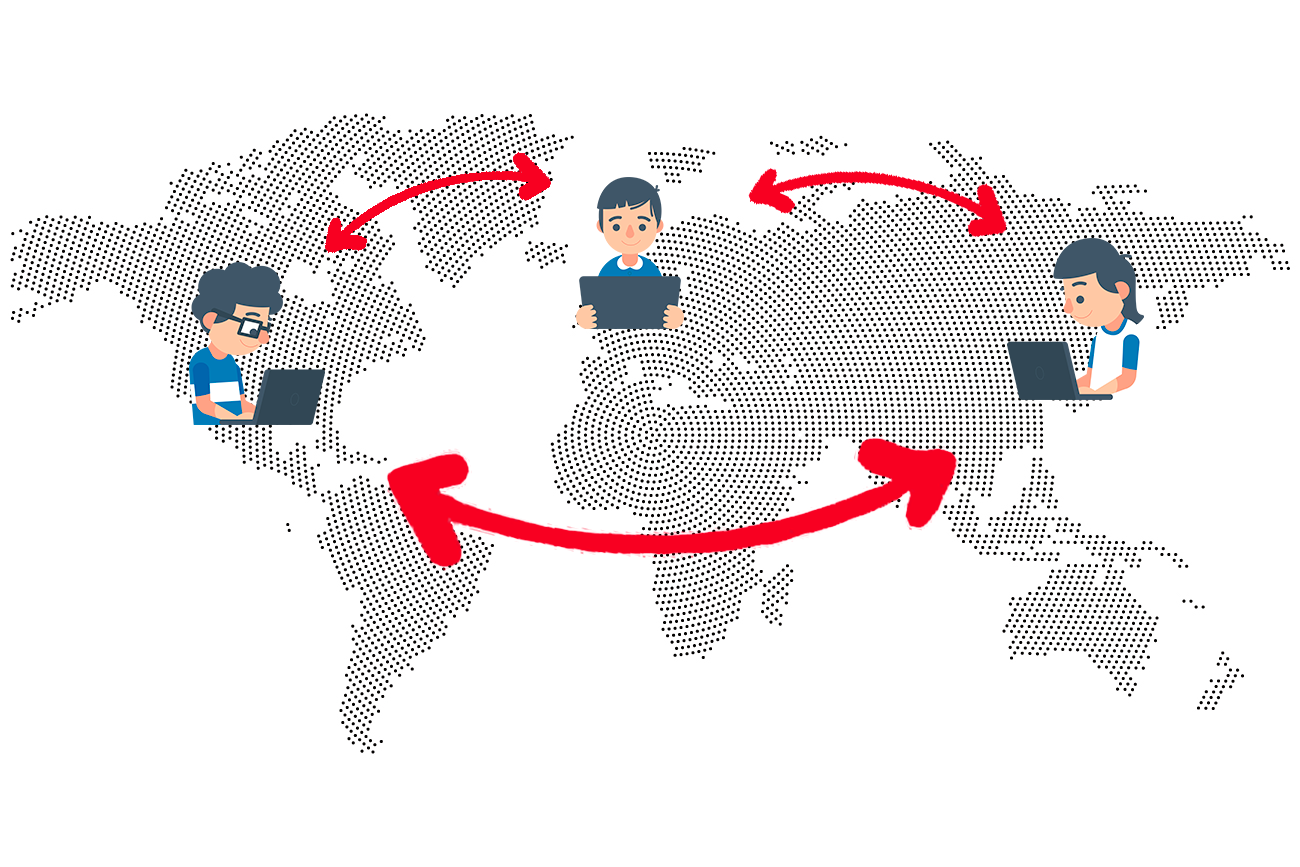
\includegraphics[width=0.75\linewidth]{DGSFiguraMapa}
	\caption[Colaboración mundial en el DGS]{En el DGS diferentes equipos de desarrollo colaboran a nivel mundial en un mismo proyecto}
	\label{fig:DGSFiguraMapa}
\end{figure} 

Gradualmente, esta tendencia esta cogiendo cada vez más fuerza en el campo de la ingeniería del software, considerándose una norma en el desarrollo de software \cite{bosnic2019assessing}. Esto es debido a que las organizaciones pueden conseguir grandes beneficios utilizando este nuevo modelo de desarrollo, ya que la principal ganancia que se consigue con su uso es la reducción en el coste económico de los proyectos, debido a que se suelen buscar territorios donde la mano de obra cualificada es barata y fácilmente disponible \cite{monasor2010preparing}. Además, se pueden encontrar otros beneficios notables como pueden ser el acercamiento del desarrollo del software al cliente y al mercado local, la reducción del período necesario para el desarrollo del software al maximizar la productividad y la expansión hacia la inclusión de trabajadores mayormente cualificados en sus actividades de desarrollo \cite{aagerfalk2008benefits}.

Sin embargo, acompañando a las anteriores ventajas que se pueden conseguir con los proyectos DGS, existen una serie de inconvenientes, los cuales son causados, principalmente, a las diferencias existentes en este tipo de proyectos las cuales podemos dividir en cuatro clases: las \emph{diferencias lingüísticas}, la \emph{distancia geográfica}, la \emph{diferencia cultural} y la coexistencia de diferentes \emph{zonas horarias}; haciendo mucho más difícil el consenso y entendimiento común \cite{monasor2010preparing}. Estas diferencias acentúan la problemática de administrar y gestionar un proyecto software, apareciendo así los tres principales desafíos en la gestión de proyectos DGS (fig.~\ref{fig:desafiosDGS}), también llamado en \cite{piattini2014desarrollo} como las 3 ces:
\begin{itemize}
	\item Desafíos en la comunicación. Los equipos de trabajo deben mantener una comunicación adecuada y activa, con el fin de llevar a cabo un intercambio constante de información y conocimientos. 
	\item Desafíos en la coordinación. Las tareas deben estar sincronizadas, para no sufrir retrasos y alcanzar objetivos e intereses comunes. 
	\item Desafíos en el control. El proyecto debe ser gestionado constantemente y confirmar que se cumplen fechas de entrega, estándares, presupuestos, etc.; además de solventar posibles contratiempos que puedan ocurrir durante el ciclo de vida del proyecto. 
\end{itemize}

\begin{figure}[htb]
	\centering
	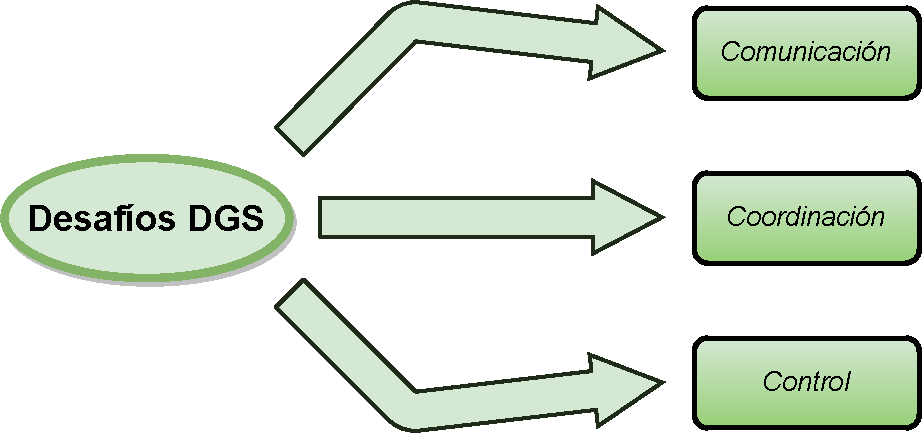
\includegraphics[width=0.75\linewidth]{desafiosDGS}
	\caption[Desafíos en los proyectos DGS]{Los tres principales desafíos en la gestión de proyectos DGS}
	\label{fig:desafiosDGS}
\end{figure}

Estos inconvenientes y desafíos complican la gestión de este tipo de proyectos, lo que puede implicar en retrasos de tareas o incluso en la cancelación del mismo, ya que según la literatura, la mayoría de proyectos DGS terminan fracasando. Según \cite{lino2015project}, la principal causa del elevado fracaso de estos proyectos es debido a la imperfecta y dificultosa gestión de los mismos. Es por esto, que para conseguir los beneficios que nos ofrece el DGS es necesario que los jefes de proyecto posean grandes conocimientos y experiencia en la gestión de estos proyectos, además de contar con una serie de habilidades (no solo técnicas, sino también no técnicas), para hacer frente a los posibles contratiempos que puedan ocurrir en el ciclo de vida del proyecto y conseguir la finalización exitosa del mismo.


\section{Propuesta}
\label{sec:Propuesta}

Como se ha indicado en la sección anterior, existe una gran problemática con la nueva tendencia de desarrollar software mediante un entorno global, debido a que un elevado número de proyectos que utilizan este tipo de modelo de desarrollo terminan fracasando, y son escasos aquellos que consiguen finalizar exitosamente, obteniéndose así los beneficios que se consiguen frente al modelo de desarrollo tradicional. Esta situación se debe, en especial, a que la educación en actividades para enseñar conocimientos sobre DGS no se está teniendo en cuenta, lo que implica que futuros ingenieros de software no posean ciertas habilidades y capacidades necesarias para afrontar los desafíos que conllevan los proyectos DGS \cite{monasor2010preparing}. Es evidente que este modelo de desarrollo se termine convirtiendo en un estándar, por lo que es necesario entrenar a nuestros estudiantes de ingeniería de software para afrontar estas dificultades, ya que se terminarán convirtiendo en los futuros ingenieros de DGS \cite{beecham2017best}.

La gestión y administración es el pilar principal sobre el que gira un proyecto, y en especial un proyecto DGS, ya que es necesaria la organización de un gran número de trabajadores y equipos de desarrollo, a los que se le añade la problemática de gestionar diferentes factores a tener en cuenta como la separación geográfica, la cultura de los diferentes países involucrados en el proyecto o el horario de trabajo en cada país, es por esto que gestionar este tipo de proyectos eficientemente, es un autentico reto. Por lo tanto, es evidente la necesidad de que existan jefes de proyecto altamente cualificados en la gestión de proyectos DGS, para que puedan afrontar la administración del mismo con éxito, solventando todos los impedimentos que puedan ocasionarse. Sin embargo, en la actualidad es complicado encontrar a jefes de proyectos DGS altamente cualificados, con una gran experiencia y con los conocimientos y habilidades necesarias para afrontar correctamente su trabajo. Como consecuencia, son muchas las organizaciones y artículos que han demandado la carencia de habilidades y experiencia en los jefes de proyecto DGS, como la principal causa del elevado nivel de fracaso en los mismos \cite{lino2015project}.

Por consiguiente, es notoria la necesidad de que existan programas de educación que enseñen a nuestro futuros ingenieros de software conocimientos sobre DGS en general, y habilidades (tanto técnicas como no técnicas) necesarias para afrontar con éxito la gestión de este tipo de proyectos en particular. En contraposición, llevar a cabo el entrenamiento y enseñanza de estas habilidades y conocimientos no es una tarea sencilla, puesto que se precisaría la necesidad de introducir a ingenieros de software inexpertos en proyectos reales (para que adquieran esa experiencia necesaria) y por consiguiente las compañías no estén dispuestas a invertir sus recursos en este tipo de programas de entrenamiento. Esta posición de las compañías es debido a que se pueden poner en riesgo proyectos en curso, además de resultar complejo reproducir un escenario real en un entorno de educación \cite{monasor2010preparing}.

En cualquier caso, hay diferentes formas de llevar a cabo la educación de diferentes conocimientos prácticos y el entrenamiento de ciertas habilidades, sin que esto pueda afectar, en nuestro caso, a un proyecto real. En el campo de la \emph{Educación en la Ingeniería de Software} se han realizado avances, buscando la manera más efectiva de educar ciertos conocimientos a estudiantes de ingeniería de software, apareciendo métodos tradicionales como proyectos finales, combinación de diferentes técnicas de enseñanza como aprendizaje basado en proyectos \cite{alabbadi2016proposed}, innovadoras estrategias como las clases volteadas \cite{choi2013applying}, o darle un enfoque relacionado con el uso de juegos, apareciendo el termino de \emph{Gamificación} \cite{connolly2007application}.

Dentro de la gamificación podemos encontrar diferentes tendencias como pueden ser: los cursos académicos \cite{murphy2008distance}, los entornos de aprendizaje \cite{burnell2002teaching} o las aplicaciones que presentan escenarios reales, conocidos como \emph{Juegos Serios} (JSs) \cite{meneely2009preparing}. En especial, los JSs (también llamados juegos educativos), según \cite{calderon2018multivocal}, consisten en juegos que van más allá del puro entretenimiento y constituyen una potente herramienta que permite a sus jugadores experimentar y aprender de sus errores, adquiriendo así experiencia y conocimientos. Los JSs ayudarán en el proceso de aprendizaje mediante la simulación de entornos virtuales, sin el riesgo que conllevaría tener al estudiante en un entorno real \cite{lino2015project, beecham2017best, calderon2018multivocal}, además de que la tendencia del desarrollo de JSs ha tenido una gran aceptación en la última década.

Como resultado de lo cual, este \emph{Trabajo Fin de Carrera} (TFG) se centrará en el desarrollo de un JS, llamado \emph{GLOBAL-MANAGER}. El objetivo de GLOBAL-MANAGER será el de ayudar a estudiante en ingeniería de software a adquirir y entrenar ciertas habilidades (en especial aquellas no técnicas también llamadas \emph{soft skills}) necesarias cuando se aborda el papel de jefe de proyecto DGS. El jugador tendrá que abordar la gestión de un proyecto DGS ficticio desde el comienzo hasta la entrega del producto software al cliente, tratando de resolver los diferentes impedimentos que se puedan ocasionar en el ciclo de vida. De esta manera, los jugadores podrán adquirir experiencia de una manera sencilla, barata e independiente, permitiéndoles afrontar con éxito un futuro trabajo en la gestión de un proyecto DGS.

Este TFG se enmarca dentro de un contrato I+D con el grupo de investigación Alarcos\footnote{\url{https://alarcos.esi.uclm.es}} de la Universidad de Castilla La-Mancha (UCLM)\footnote{\url{https://www.uclm.es/}}, en concreto en el proyecto "G3SOFT: Ingeniería de Modelos para el Gobierno y Gestión del Desarrollo Global de Software"\footnote{\url{https://alarcos.esi.uclm.es/proyectos/G3SOFT/index.php}}, el cual se centra en la mejora del gobierno y la gestión de proyectos de DGS. En la tab.~\ref{tab:ResumenG3SOFT} se muestra un resumen de dicho proyecto.

\begin{table}[htbp]
	\centering
	\setlength{\arrayrulewidth}{0.5mm}
	\arrayrulecolor{white}
	\resizebox{\textwidth}{!}{
    \begin{tabular}{l | p{25.5em}}
        \rowcolor[rgb]{.082, .082, .565} \textcolor[rgb]{1, 1, 1}{\textbf{Nombre:}} & \cellcolor[rgb]{.753, .753, .753}G3SOFT:Ingeniería de Modelos para el Gobierno y Gestión del\newline{}Desarrollo Global de Software \\ \hline
        \rowcolor[rgb]{.082, .082, .565} \textcolor[rgb]{1, 1, 1}{\textbf{Financiación:}} & \cellcolor[rgb]{.753, .753, .753}JJCM Consejería de Educación y Cultura y Deportes, y Fondos\newline{}FEDER \\ \hline
        \rowcolor[rgb]{.082, .082, .565} \textcolor[rgb]{1, 1, 1}{\textbf{Referencia:}} & \multicolumn{1}{l}{\cellcolor[rgb]{.753, .753, .753}SBPLY/17/180501/000150} \\ \hline
        \rowcolor[rgb]{.082, .082, .565} \textcolor[rgb]{1, 1, 1}{\textbf{Dirección WEB:}} & \multicolumn{1}{l}{\cellcolor[rgb]{.753, .753, .753}\url{https://alarcos.esi.uclm.es/proyectos/G3SOFT/index.php}} \\ \hline
        \rowcolor[rgb]{.082, .082, .565} \textcolor[rgb]{1, 1, 1}{\textbf{Grupo de investigación:}} & \multicolumn{1}{l}{\cellcolor[rgb]{.753, .753, .753}Grupo Alarcos} \\ \hline
        \rowcolor[rgb]{.082, .082, .565} \textcolor[rgb]{1, 1, 1}{\textbf{Universidad colaboradora:}} & \multicolumn{1}{l}{\cellcolor[rgb]{.753, .753, .753}Universidad de Castilla-La Mancha (UCLM)} \\ \hline
    	\rowcolor[rgb]{.082, .082, .565} \textcolor[rgb]{1, 1, 1}{\textbf{Investigadores principales:}} & \cellcolor[rgb]{.753, .753, .753}Francisco Ruiz Gónzalez\newline{}Aurora Vizcaíno Barceló \\ \hline
    \end{tabular}}
	\caption{Resumen del proyecto G3SOFT}
	\label{tab:ResumenG3SOFT}
\end{table}

\section{Estructura del documento}
\label{sec:Estructura}
\end{document}